\documentclass{article}\usepackage[]{graphicx}\usepackage[]{color}
%% maxwidth is the original width if it is less than linewidth
%% otherwise use linewidth (to make sure the graphics do not exceed the margin)
\makeatletter
\def\maxwidth{ %
  \ifdim\Gin@nat@width>\linewidth
    \linewidth
  \else
    \Gin@nat@width
  \fi
}
\makeatother

\definecolor{fgcolor}{rgb}{0.345, 0.345, 0.345}
\newcommand{\hlnum}[1]{\textcolor[rgb]{0.686,0.059,0.569}{#1}}%
\newcommand{\hlstr}[1]{\textcolor[rgb]{0.192,0.494,0.8}{#1}}%
\newcommand{\hlcom}[1]{\textcolor[rgb]{0.678,0.584,0.686}{\textit{#1}}}%
\newcommand{\hlopt}[1]{\textcolor[rgb]{0,0,0}{#1}}%
\newcommand{\hlstd}[1]{\textcolor[rgb]{0.345,0.345,0.345}{#1}}%
\newcommand{\hlkwa}[1]{\textcolor[rgb]{0.161,0.373,0.58}{\textbf{#1}}}%
\newcommand{\hlkwb}[1]{\textcolor[rgb]{0.69,0.353,0.396}{#1}}%
\newcommand{\hlkwc}[1]{\textcolor[rgb]{0.333,0.667,0.333}{#1}}%
\newcommand{\hlkwd}[1]{\textcolor[rgb]{0.737,0.353,0.396}{\textbf{#1}}}%

\usepackage{framed}
\makeatletter
\newenvironment{kframe}{%
 \def\at@end@of@kframe{}%
 \ifinner\ifhmode%
  \def\at@end@of@kframe{\end{minipage}}%
  \begin{minipage}{\columnwidth}%
 \fi\fi%
 \def\FrameCommand##1{\hskip\@totalleftmargin \hskip-\fboxsep
 \colorbox{shadecolor}{##1}\hskip-\fboxsep
     % There is no \\@totalrightmargin, so:
     \hskip-\linewidth \hskip-\@totalleftmargin \hskip\columnwidth}%
 \MakeFramed {\advance\hsize-\width
   \@totalleftmargin\z@ \linewidth\hsize
   \@setminipage}}%
 {\par\unskip\endMakeFramed%
 \at@end@of@kframe}
\makeatother

\definecolor{shadecolor}{rgb}{.97, .97, .97}
\definecolor{messagecolor}{rgb}{0, 0, 0}
\definecolor{warningcolor}{rgb}{1, 0, 1}
\definecolor{errorcolor}{rgb}{1, 0, 0}
\newenvironment{knitrout}{}{} % an empty environment to be redefined in TeX

\usepackage{alltt}
\usepackage[margin=1.0in]{geometry}
\usepackage[colorlinks=true,urlcolor=darkblue,linkcolor=greenteal]{hyperref}  %This makes reference links hyperlinks in pdf (tip from

\usepackage[parfill]{parskip}    % Activate to begin paragraphs with an empty line rather than an indent (tip from Revelle's 'psych' package).

\definecolor{darkblue}{rgb}{.0,.2,.8}
\definecolor{greenteal}{rgb}{0,.5,.5}

\title{The NLS Investigator}
\author{
  \href{http://scholar.google.com/citations?user=ffsJTC0AAAAJ}{William Howard Beasley} (\href{http://howardliveoak.com/}{Howard Live Oak LLC}, Norman)\\
  \href{http://www.vanderbilt.edu/psychological_sciences/bio/joe-rodgers}{Joseph Lee Rodgers} (Vanderbilt University, Nashville)\\
  \href{http://find.ouhsc.edu/Faculty.aspx?FacultyID=1041}{David Bard} (University of Oklahoma Health Sciences Center, OKC)\\
  Kelly Meredith (University of Oklahoma, Norman)\\
  \href{http://students.ou.edu/H/Michael.D.Hunter-1/}{Michael D. Hunter} (University of Oklahoma, Norman)
}
\IfFileExists{upquote.sty}{\usepackage{upquote}}{}

\begin{document}

\setkeys{Gin}{width=\textwidth}
\newcommand{\code}[1]{\texttt{\small{#1}}}
\newcommand{\pkg}[1]{\textsf{\small{#1}}}
\let\proglang=\textsf
\newcommand{\R}{\proglang{R}} %(tip from Revelle's 'psych' package).

\maketitle
\tableofcontents

\begin{abstract}
This vignette will be useful to behavior genetic researchers interested in using the National Longitudinal Survey of Youth (NLSY79) or Children (NLSYC) data.  To fit biometrical models to the NLSY or NLSYC requires that the data be extracted from the appropriate online NLSY database into a usable file format.  The extracting software is called the \href{https://www.nlsinfo.org/investigator/pages/login.jsp}{NLS Investigator}.  We describe how to use the NLS Investigator to select and download variables.   In \href{http://cran.r-project.org/web/packages/NlsyLinks/}{subsequent vignettes}, we show how to reformat the data into file structures that accommodate behavior genetic research, and how to fit biometrical models.  The following steps are not specific to \R{}, but rather precede the use of any analytic statistical software.
\end{abstract}



%%%%%%%%%%%%%%%%%%%%%%%%%%%%%%%%%%%%%%%%%%%%%%
\section{Terminology} %\label{sec:Terminology}
This package considers both generations of the NLSY79.  The first generation (\emph{ie}, `Gen1') refers to subjects in the original NLSY79 sample (\url{http://www.bls.gov/nls/nlsy79.htm}).  The second generation (\emph{ie}, `Gen2') of subjects are the biological offspring of the original females -\emph{i.e.}, those in the NLSY79 Children and Young Adults sample ( \url{http://www.bls.gov/nls/nlsy79ch.htm}).  The NLSY97 is a third dataset that can be used for behavior genetic research (\url{http://www.bls.gov/nls/nlsy97.htm}), although this vignette focuses on the two generations in the NLSY79.

Standard terminology is to refer second generation subjects as `children' when they are younger than age 15 (NSLYC), and as `young adults' when they are 15 and older (NLSY79-YA); though they are the same respondents, different funding mechanisms and different survey items necessitate the distinction.  This cohort is sometimes abbreviated as `NLSY79-C', `NLSY79C', `NLSY-C' or `NLSYC'. This packages uses `Gen2' to refer to subjects of this generation, regardless of their age at the time of the survey.

%%%%%%%%%%%%%%%%%%%%%%%%%%%%%%%%%%%%%%%%%%%%%%
\section{Steps to Select Variables and Download Data}
\begin{enumerate}
\item Browse to \url{http://www.nlsinfo.org/investigator/}.  Select the `REGISTER' link in the top right, and create a personal account.  If you have already registered, Log In and proceed to the next step.
\item Select your desired cohort, in the dropdown box titled, ``Select the study you want to work with:''.  In the screenshot below, second generation of the NLSY79 sample is selected.

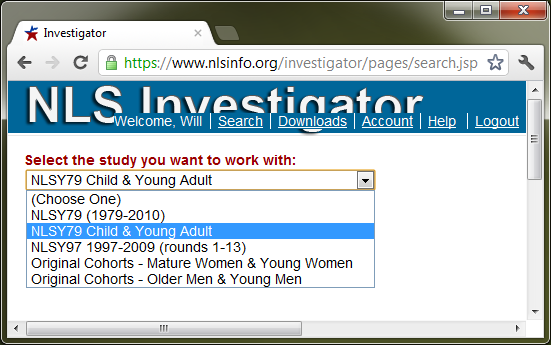
\includegraphics{D:/Projects/RDev/NlsyLinksStaging/Vignettes/NlsInvestigatorCohort.png}

\item Select the variables.  There are tens of thousands of variables in some cohorts, and selecting the correct ones can require careful attention and a few tricks.  A thorough tutorial begins on the NLS Investigator page: \url{http://www.nlsinfo.org/InvestigatorGuide/investigator_guide_TOC.html}.  To better leverage the NLSY's extensive variable set (and to avoid mistakes), we recommend that researchers dedicate time to this tutorial.  However for the purposes of this vignette, we'll simply select a few easy variables.  

First, in the `Variables Search' tab, select `Word in Title (enter search term)'.  Second, type ``other symptom - f'' in the textbox.  Third, clicking the `Display Variables' button should retrieve at least four NLSYC variables whose title starts with ``other symptom - f''.  Fourth, supposing we care about only their fevers, click their two corresponding checkboxes.  (If you're curious, the `XRND' value for year stands for \href{http://www.bls.gov/nls/nls138.pdf}{cross round}; XRND variables are calculated by the NLS staff, and typically come from the subject's most recent survey).

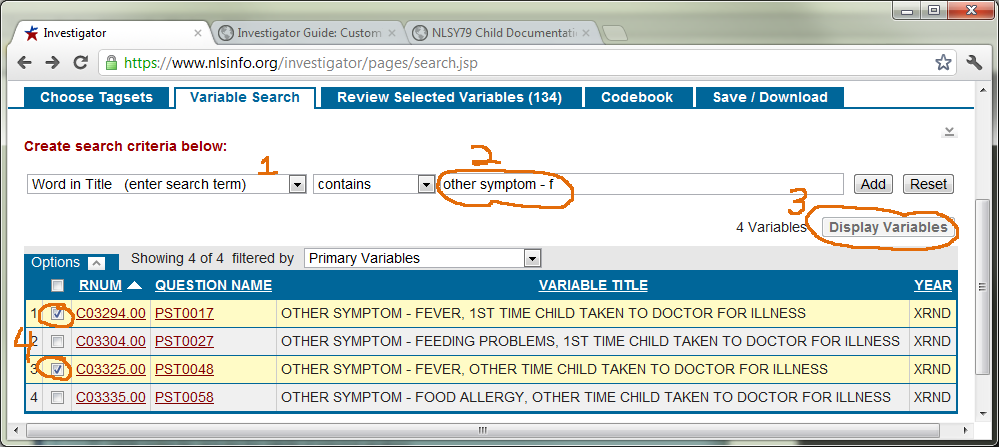
\includegraphics{D:/Projects/RDev/NlsyLinksStaging/Vignettes/NlsInvestigatorSelect.png}

\item Review your selected variables by clicking the corresponding tab.  Notice that several important variables are automatically included in every  dataset.  In real research these steps are iterated many times, as you repeated select, then review, then save, then re-select, then re-review, then...  But we'll move on, because these seven variables are good enough for an example.

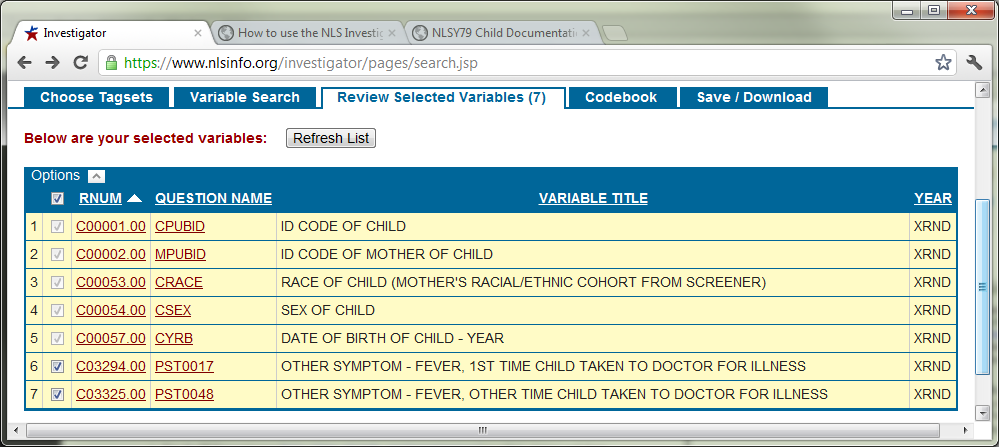
\includegraphics{D:/Projects/RDev/NlsyLinksStaging/Vignettes/NlsInvestigatorReview.png}

\item When the dataset is complete, it is time to save the tagset.  A \textbf{tagset file} is simply metadata of the desired variables.  The file identifies the variables, \emph{but does not contain actual data values}.  As your project evolves over time (because you're adding variables, or refreshing your dataset after a new survey is released), it's convenient to keep the metadata distinct from the real data.  

The actual values are contained in the \textbf{data file}, which is discussed in the next two steps.  These issues are covered further in the \href{http://www.nlsinfo.org/InvestigatorGuide/investigator_guide_TOC.html}{official tutorial}.

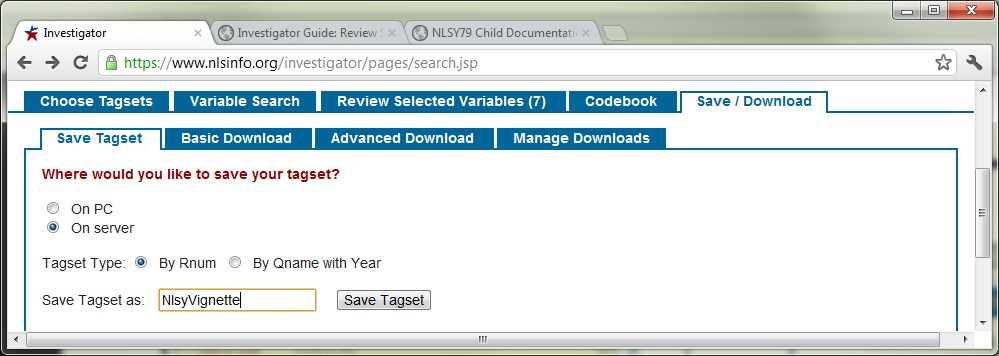
\includegraphics{D:/Projects/RDev/NlsyLinksStaging/Vignettes/NlsInvestigatorTagset.png}

\item The first step of the download process is to create the data file on the NLS server.  Click the `Save/Download' tab, and then the `Advanced Download' tab.  As far as the \pkg{NlsyLinks} package is concerned, only the the `Comma-delimited datafile...' box needs to be checked.  Then provide a `Data filename'.  Finally, click the `Start Download' button.

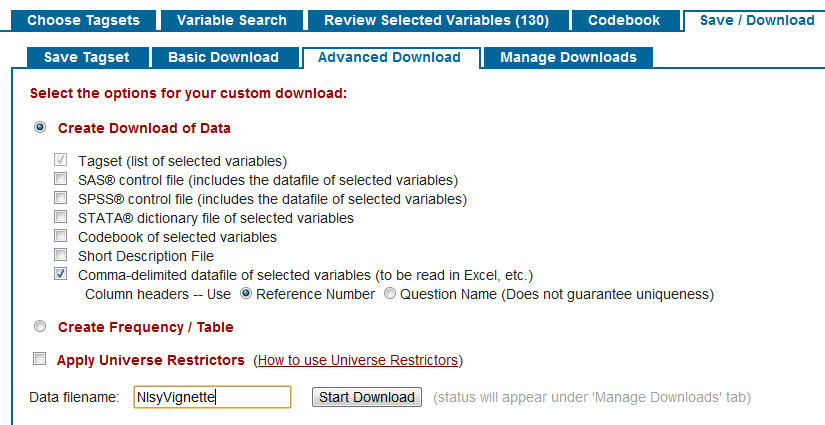
\includegraphics{D:/Projects/RDev/NlsyLinksStaging/Vignettes/NlsInvestigatorDownloadStep1.png}

\item The second step of the download process is to transfer the zip file to your local computer.  Click the maroon `download' hyperlink.

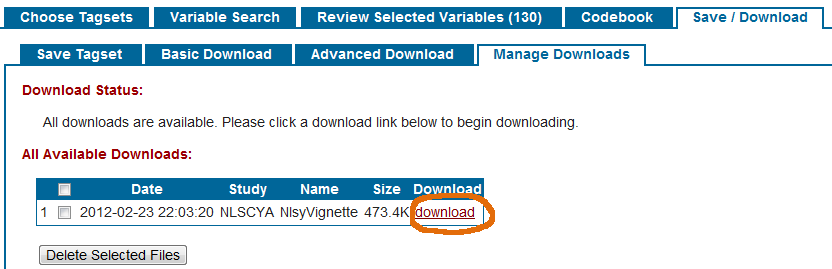
\includegraphics{D:/Projects/RDev/NlsyLinksStaging/Vignettes/NlsInvestigatorDownloadStep2.png}

\item Open the zip file and extract the *.csv file to a location that the vignette examples have permission to read.  Then try some of the \code{NlsyLinks} vignette examples at \url{http://cran.r-project.org/web/packages/NlsyLinks/}. 

\end{enumerate}
\section{Using Multiple Tagsets}
Tagsets were introduced in Step 5, but are discussed more thoroughly here.  Tagsets make large projects more manageable in two ways.  First, they save effort and reduce errors because you don't have to re-select all the variables every time you revisit the NLS Investigator.  You can save and load the tagsets during subsequent sessions.  In fact, you can save multiple tagsets on the NLS server.

Second, using \emph{multiple} tagsets provides a convenient approach to organize and compartmentalize your variables.  It's not unusual for some complicated longitudinal studies to use hundreds of NLSY variables.  We've found it easier to manage five tagsets of ~100 variables, than one tagset of 500.  Since all NLSY tagsets (and therefore their datasets) automatically include the subject ID, merging the multiple datasets later is trivial with statistical software. 

In \R{}, use the \code{merge} function; the \code{by} argument should be `R0000100' for NLSY79 subjects,  `C0000100' for NLSYC subjects, and `R0000100' for NLSY97 subjects.  For example, a study about intelligence and teenage fertility would have one tagset containing the intelligence variables, and a second tagset containing the fertility variables.  These two tagsets eventually could produce two CSV data files called \code{IQ.csv} and \code{Fertility.csv}, located in the \code{BGResearch} directory.  The \R{} code to read and merge these two datasets could be as simple as
\begin{Sinput}
dsIQ <- read.csv('C:/BGResearch/IQ.csv', header=TRUE)
dsFertility <- read.csv('C:/BGResearch/Fertility.csv', header=TRUE)
ds <- merge(dsIQ, dsFertility, by="C0000100")
\end{Sinput}

In SAS, the \code{merge} function (and its \code{BY} argument) \href{http://support.sas.com/documentation/cdl/en/basess/58133/HTML/default/viewer.htm#a001318494.htm}{behaves similarly} as above.  Notice that the SAS documentation states, ``Before you can perform a match-merge, all data sets must be sorted by the variables that you want to use for the merge", which is \code{C0000100} in this example.

If you're importing CSV files specifically for the \pkg{NlsyLinks} package, you'll find functions like \code{ReadCsvNlsy79Gen1} and \code{ReadCsvNlsy79Gen2} more convenient for later analyses.
\section{Tagset History}
We recommend saving the tagsets on both the NLS server and your local machine.  Tagsets are not guaranteed to be retained on the NLS server more than 90 days.  Locally save when variables are added or removed from the tagset in a consistent location, and name the file to reflect the current date.  The files can be read with any simple text editor.  The directory below contains the partial evolution of four distinct tagsets (i.e., `Gen1Links', `Gen2Links', `Gen2ImplicitFather', `Gen2LinksFromGen1').

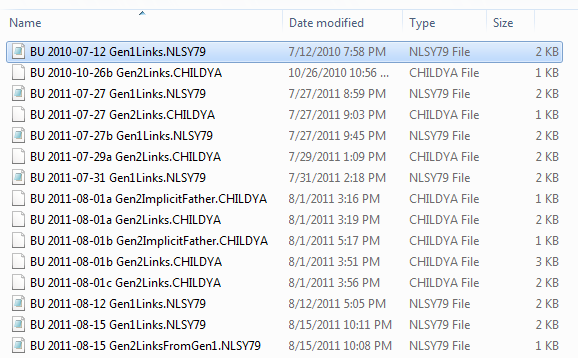
\includegraphics[width=4in]{D:/Projects/RDev/NlsyLinksStaging/Vignettes/NlsInvestigatorTagsetBackups.png}

\section{Notes}
This package's development was largely supported by the NIH Grant 1R01HD65865, \href{http://taggs.hhs.gov/AwardDetail.cfm?s_Award_Num=R01HD065865&n_Prog_Office_Code=50}{``NLSY Kinship Links: Reliable and Valid Sibling Identification"} (PI: Joe Rodgers; Vignette Construction by Will Beasley)\\


These screenshots were taken February and March 2012 with Google Chrome 17 and Windows 7 SP1 Enterprise.  If you notice something that no longer corresponds to the current version to the NLS Investigator, please tell us.
\end{document}
